%----------------------------------------------------------------------------
\chapter{Tesztelés}
\label{sec:testing}
%----------------------------------------------------------------------------
%----------------------------------------------------------------------------

A \figref{APBwrite} ábrán látható egy szimulációs hullámforma, amely a helyes APB vezérlőjel dekódolást hivatott demonstrálni. A kurzorral megjelölt hely előtti PCLK felfutóélre már minden szükséges vezérlő és engedélyezőjel ki volt adva az APB master részéről, az APB modul mégsem küld semmiféle adatot az I2C modul felé, mivel a PADDR buszon kiadott cím nem egyezik a perifériánk 0x80000000 címével. Viszont az ábrán 675ns - nál megfigyelhető egy helyes címre történő írás, így az A2I vezetéken megjelenik PWDATA tartalma, amit az I2C modul fel is dolgoz, és kezdi is a kommunikációt.
\begin{figure}[ht!]
    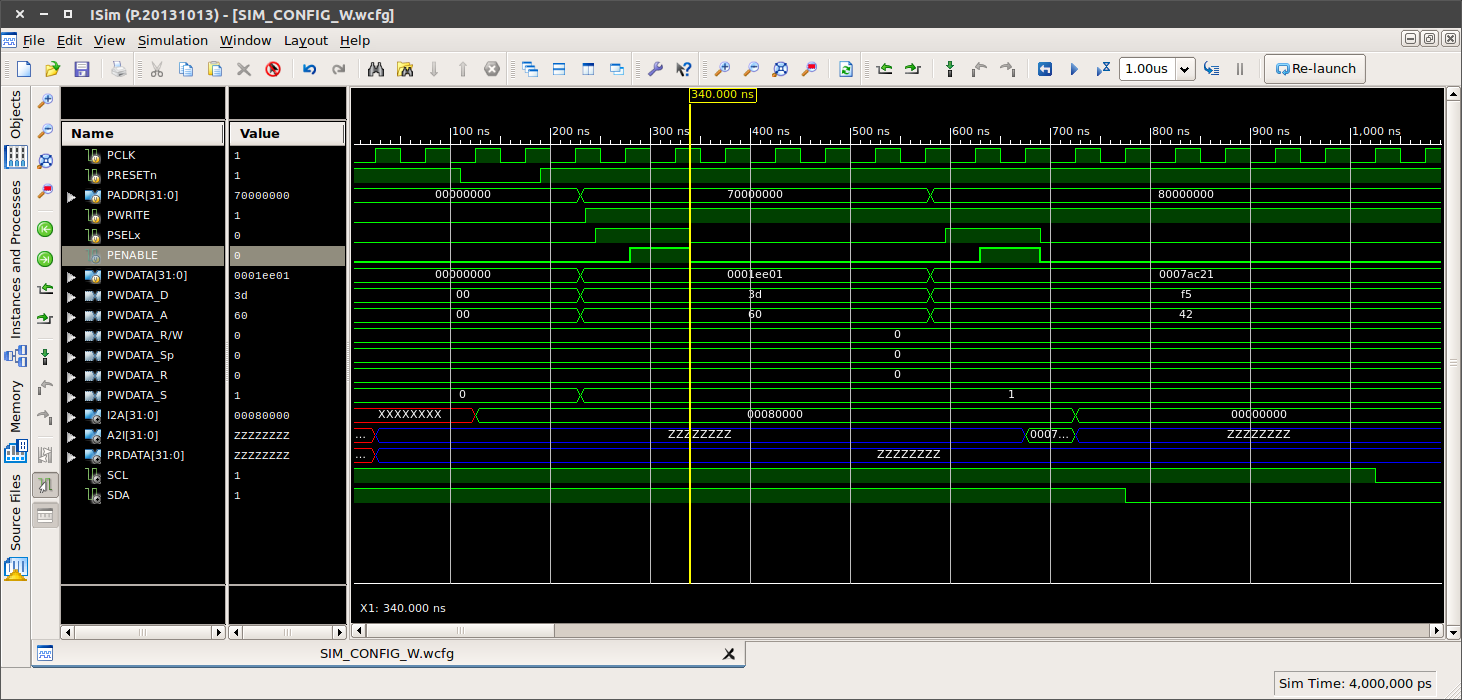
\includegraphics[width=\textwidth]{figures/APB_invalidwrite.png}
    \caption{APB írás ciklus}
    \label{fig:APBwrite}
\end{figure}

A szimulációt tovább futtatva megfigyelhetünk egy rendben lezajló I2C írásmúveletet a \figref{I2Cwrite} ábrán. A szimulációhoz a slave felől érkező ACK jeleket kézzel, a szimulációs fájlokban szereplő módon adtuk ki, hogy igazolhassuk a modul megfelelő működését. A fájl természetesen megtalálható az \ref{tbtopW} függelékben.
A hullámforma egy byte-nyi 0xF5 adat 0x42 címre történő írását ábrázolja.
\begin{figure}[ht!]
    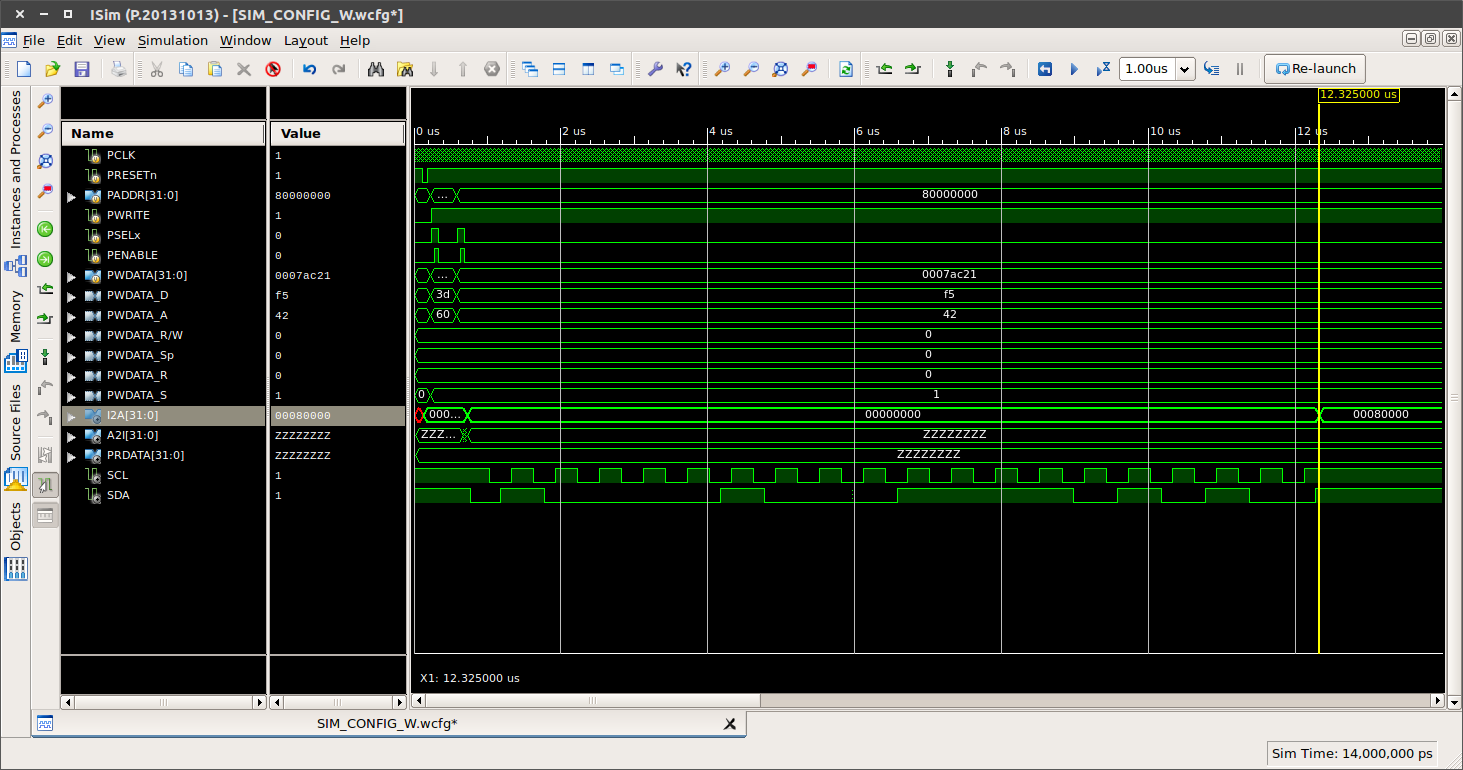
\includegraphics[width=\textwidth]{figures/I2C_W2.png}
    \caption{I2C írás ciklus}
    \label{fig:I2Cwrite}
\end{figure}

A következő, \figref{I2Cread} ábrán egy I2C olvasási ciklust szimuláltunk. Az ehhez tartozó szimulációs fájl szintén megtalálható a \ref{tbtopR} függelékben.
Megfigyelhető egy lekérdezés az átvitel közben, de az olvasott adat ekkor \textbf{RDY} bit hiányában érvénytelen. Még egy APB olvasás látható a hullámformán, ezúttal már az átvtel lezajlása után, mikor is megfigyelhető az I2A, illetve a PRDATA buszokon az SDA vonalra kézzel felvezetett 0xC5 adat.
\begin{figure}[ht!]
    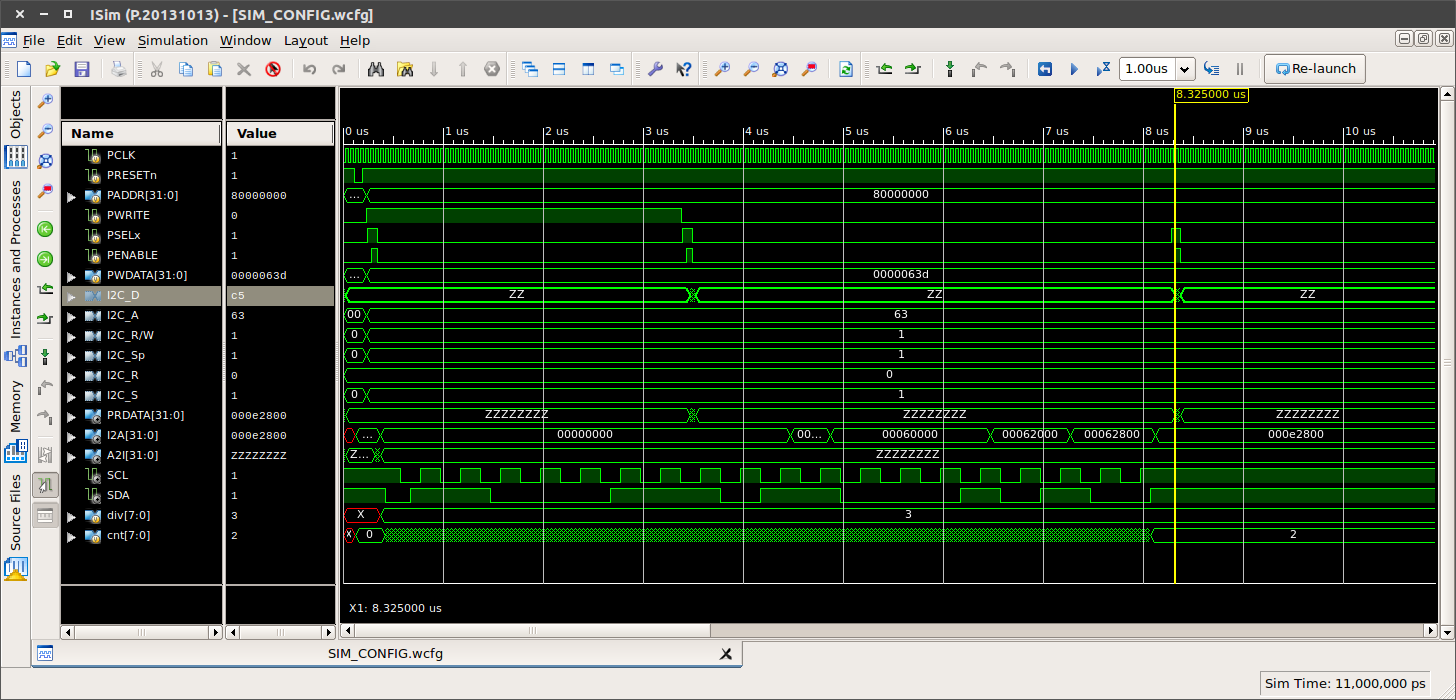
\includegraphics[width=\textwidth]{figures/I2C_R4.png}
    \caption{I2C olvasás ciklus}
    \label{fig:I2Cread}
\end{figure}
